\documentclass[11pt]{article}

\usepackage{hyperref}
\usepackage{amsfonts,amsmath,amssymb,amsthm}
\usepackage{epsfig, graphics, graphicx}
\usepackage{latexsym}
\usepackage{fullpage}
\usepackage[parfill]{parskip}
%\usepackage{mysymbols}
\usepackage[tight]{subfigure}
\usepackage{hyperref}
\usepackage{enumerate,comment}
\usepackage{float}

\newcommand{\figref}[1]{Fig.~\ref{#1}}
\newcommand{\R}{\mathbb{R}}

\begin{document}
Shashank Singh\footnote{sss1@andrew.cmu.edu}
\setcounter{section}{2}
\section{Newton and quasi-Newton methods [25 points] (Sashank)}
\begin{enumerate}[(a)]
\item See Figure~\ref{fig:3a}.
\begin{figure}[h]
\centering
\begin{tabular}{cc}
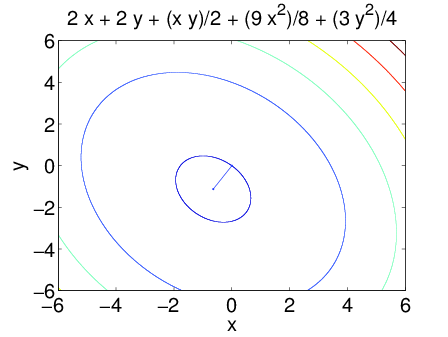
\includegraphics[width=200pt,height=150pt]{3a1}   &
    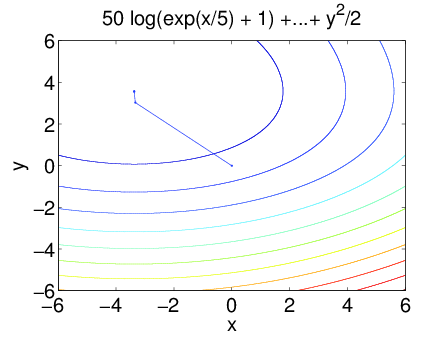
\includegraphics[width=200pt,height=150pt]{3a2}  \\
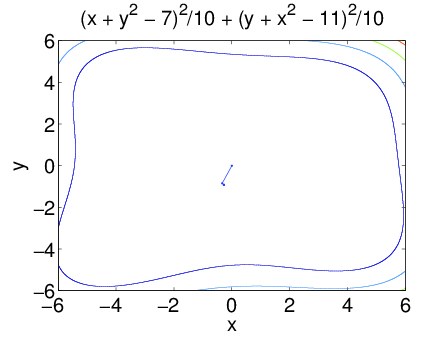
\includegraphics[width=200pt,height=150pt]{3a3}   &
    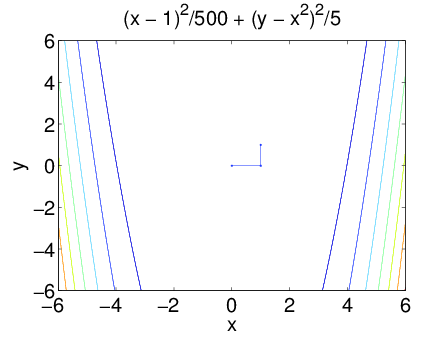
\includegraphics[width=200pt,height=150pt]{3a4}
\end{tabular}
\caption{Trajectories of Newton's Method (starting at $(0,0)$) and contour
plots of each function.}
\label{fig:3a}
\end{figure}

\item See Figure~\ref{fig:3b}.
\begin{figure}[h]
\centering
\begin{tabular}{cc}
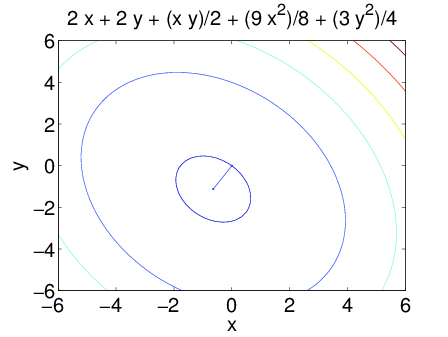
\includegraphics[width=200pt,height=150pt]{3b1}   &
    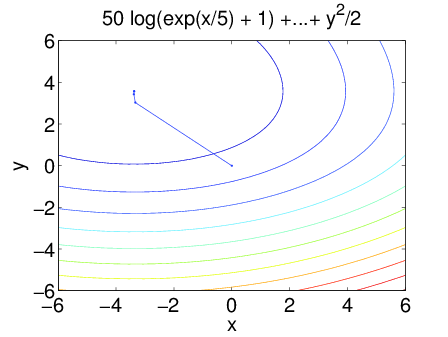
\includegraphics[width=200pt,height=150pt]{3b2}  \\
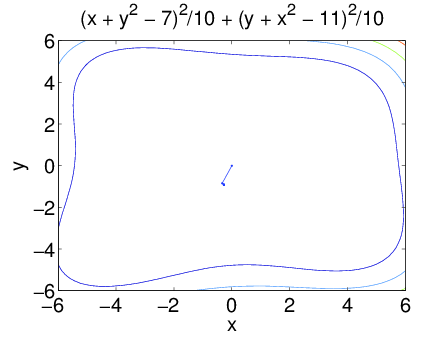
\includegraphics[width=200pt,height=150pt]{3b3}   &
    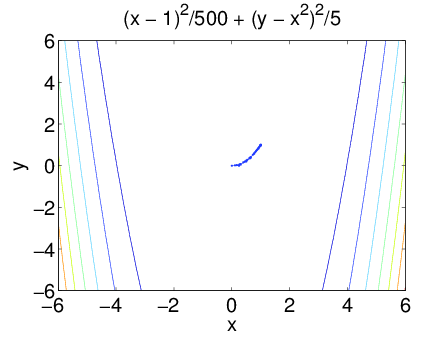
\includegraphics[width=200pt,height=150pt]{3b4}
\end{tabular}
\caption{Trajectories of the BFGS algorithm (starting at $(0,0)$) and contour
plots of each function.}
\label{fig:3b}
\end{figure}

\item The final points, and hence the function values, are the same for both
algorithms (see Tables~\ref{tab:3c1},\ref{tab:3c2}, and \ref{tab:3c3}), except
on $f_H$ starting at $(2,2)$. This makes sense, because $f_H$ is the most
obviously non-convex of the $4$ functions. Examining the trajectory of Newton's
method in this case shows that it very quickly shoots off far from the closest
minimum before converging to another minimum. Backtracking prevents this from
happening with BFGS.
\begin{table}
\centering
\begin{tabular}[h]{lcccc}
Function  & Newton final point    & BFGS final point        & Newton function value & BFGS function value   \\
\hline
$f_Q$     & $(-0.6400,  -1.1200)$ & $(-0.6400,   -1.1200)$  & $   -1.7600$          & $ -1.7600$            \\
$f_{LL}$  & $(-3.3742,   3.5787)$ & $(-3.3742,    3.5787)$  & $   40.4012$          & $ 40.4012$            \\
$f_H$     & $(-0.2708,  -0.9230)$ & $(-0.2708,   -0.9230)$  & $   18.1617$          & $ 18.1617$            \\
$f_R$     & $( 1.0000,   1.0000)$ & $( 1.0000,    1.0000)$  & $         0$          & $  0.0000$
\end{tabular}
\caption{Final values and functions values for each algorithm and
function, starting from $(0,0)$.}
\label{tab:3c1}
\end{table}

\begin{table}
\centering
\begin{tabular}[h]{lcccc}
Function  & Newton final point    & BFGS final point        & Newton function value & BFGS function value   \\
\hline
$f_Q$     & $(-0.6400,  -1.1200)$ & $(-0.6400,   -1.1200)$  & $   -1.7600$          & $ -1.7600$            \\
$f_{LL}$  & $(-3.3742,   3.5787)$ & $(-3.3742,    3.5787)$  & $   40.4012$          & $ 40.4012$            \\
$f_H$     & $( 3.5844,  -1.8481)$ & $( 3.0000,    2.0000)$  & $    0.0000$          & $  0.0000$            \\
$f_R$     & $( 1.0000,   1.0000)$ & $( 1.0000,    1.0000)$  & $         0$          & $  0.0000$
\end{tabular}
\caption{Final values and functions values for each algorithm and
function, starting from $(2,2)$.}
\label{tab:3c2}
\end{table}

\begin{table}
\centering
\begin{tabular}[h]{lcccc}
Function  & Newton final point    & BFGS final point        & Newton function value & BFGS function value   \\
\hline
$f_Q$     & $(-0.6400,  -1.1200)$ & $(-0.6400,   -1.1200)$  & $-1.7600$          & $ -1.7600$            \\
$f_{LL}$  & $(-3.3742,   3.5787)$ & $(-3.3742,    3.5787)$  & $40.4012$          & $ 40.4012$            \\
$f_H$     & $( 3.0000,   2.0000)$ & $( 3.0000,    2.0000)$  & $ 0.0000$          & $  0.0000$            \\
$f_R$     & $( 1.0000,   1.0000)$ & $( 1.0000,    1.0000)$  & $      0$          & $  0.0000$
\end{tabular}
\caption{Final values and functions values for each algorithm and
function, starting from $(3,3)$.}
\label{tab:3c3}
\end{table}

\item On $f_Q$, $f_{LL}$, and $f_H$, the number of iterations for both
algorithms are comparable (differing by at most 2; see Table~\ref{tab:3d}).
It's possible that the starting positions are simply too close to the optima to
notice a difference. However, for $f_R$, BFGS consistently requires many more
iterations than Newton's method. Iterations of Newton's method are generally
$O(n^p)$, for some $p \in [2.3,3])$ (due to the inversion of the $n \times n$
Hessian). The most expensive operations in an iteration of BFGS are several
multiplications of $n$-dimensional vectors by $n \times n$ matrices, requiring
$O(n^2)$ time.

\begin{table}
\centering
\begin{tabular}[h]{lcccc}
Function    & Newton iterations     & BFGS iterations       & Newton iterations     & BFGS iteration        \\
            & starting at $(0,0)$   & starting at $(0,0)$   & starting at $(2,2)$   & starting at $(2,2)$   \\
\hline
$f_Q$       & 2                     & 2                     & 2                     & 2                     \\
$f_{LL}$    & 5                     & 7                     & 5                     & 6                     \\
$f_H$       & 5                     & 7                     & 9                     & 9                     \\
$f_R$       & 3                     & 37                    & 6                     & 44                    \\
\hline
            & Newton iterations     & BFGS iterations       &                       &                       \\
            & starting at $(3,3)$   & starting at $(3,3)$   &                       &                       \\
\hline
$f_Q$       & 2                     &  2                    &                       &                       \\
$f_{LL}$    & 4                     &  6                    &                       &                       \\
$f_H$       & 6                     &  8                    &                       &                       \\
$f_R$       & 6                     & 52                    &                       &                       \\
\end{tabular}
\caption{Number of iterations for each algorithm and function, at various
starting points.}
\label{tab:3d}
\end{table}
\end{enumerate}
\end{document}
